%qqqqqqqqqqqqqqqqqqqqqqqqqqqqqqqqqqqqqqqqqqqqqqqqqqqqqqqqqqqqqqqqqqqqqqqqq
%Quote
\begin{savequote}[50mm]
%‘‘El cosmos es todo lo que es, todo lo que fue y todo lo que será. Nuestras 
%más ligeras contemplaciones del cosmos nos hacen estremecer: Sentimos como 
%un cosquilleo nos llena los nervios, una voz muda, una ligera sensación como
%de un recuerdo lejano o como si cayéramos desde gran altura. Sabemos que nos
%aproximamos al más grande de los misterios.’’
%\qauthor{Carl Sagan}
\end{savequote}
%qqqqqqqqqqqqqqqqqqqqqqqqqqqqqqqqqqqqqqqqqqqqqqqqqqqqqqqqqqqqqqqqqqqqqqqqq




%#########################################################################
\chapter{Alineamiento de AGNs con su entorno a gran escala}
\label{cha:cosmic_web}

En esta sección se presentan los resultados obtenidos en la búsqueda de posible alineamiento del espín de los AGNs y el entorno cosmológico al cual pertenecen. Con al fin de poder llevar a cabo este propósito, se hace uso de: dos simulaciones cosmológicas ({\it{Cosmo01}} y {\it{Cosmo02}}), los los autovalores, autovectores, sobre densidades obtenidos con el método de T-Web y el catálogo FoF. A continuación se presentan las características de la simulaciones y de los resultados obtenidos.

%------------------------------------------------
\section{Características de las simulaciones}
\label{sec: propiedades en las simulaciones}
%------------------------------------------------

En la simulación hay parámetros o valores que dan información de la dinámica del sistema,  que arrojan criterios suficientes para decidir si lo obtenido está en acuerdo con los modelos físicos propuestos. 
Conforme a esto, se pretende realizar un análisis a la distribución de masa (función de masa) de los halos de materia, BHs y de estrellas. 

Debido a que no todos los halos hospedan un BH en su interior, fue necesario descartar los halos que no cumplen con esta condición. Esto reduce de gran manera la cantidad de galaxias a estudiar, sin embargo es suficiente para realizar un análisis adecuado.

%------------------------------------------------
    \subsection{ Función de masa}
    \label{subsec: funcion de masa}
%------------------------------------------------
La función de masa es uno de los parámetros de control más contundentes en el análisis de las simulaciones. Bajo la teoría de formación y evolución de galaxias se tiene que los objetos con baja masa son más abundantes, debido a que en los procesos evolutivos de las galaxias la interacción es jerárquica, las galaxias más masivas tiene una mayor probabilidad en fusionarse con otras debido a su gran potencial gravitacional, esto hace que las galaxias más densas se terminen fusionando y disminuyendo su población. Con base a esto la función de masa de las galaxias (halos, BHs y masa estelar) debe decrecer a medida que se aumentan las masas, i.e., La cantidad de objetos disminuye a medida que aumenta la masa, es menos probable encontrar BHs muy masivos.

%
\begin{figure}
 \centering
  \subfloat{
   %\label{fig: función de masa BHs}
    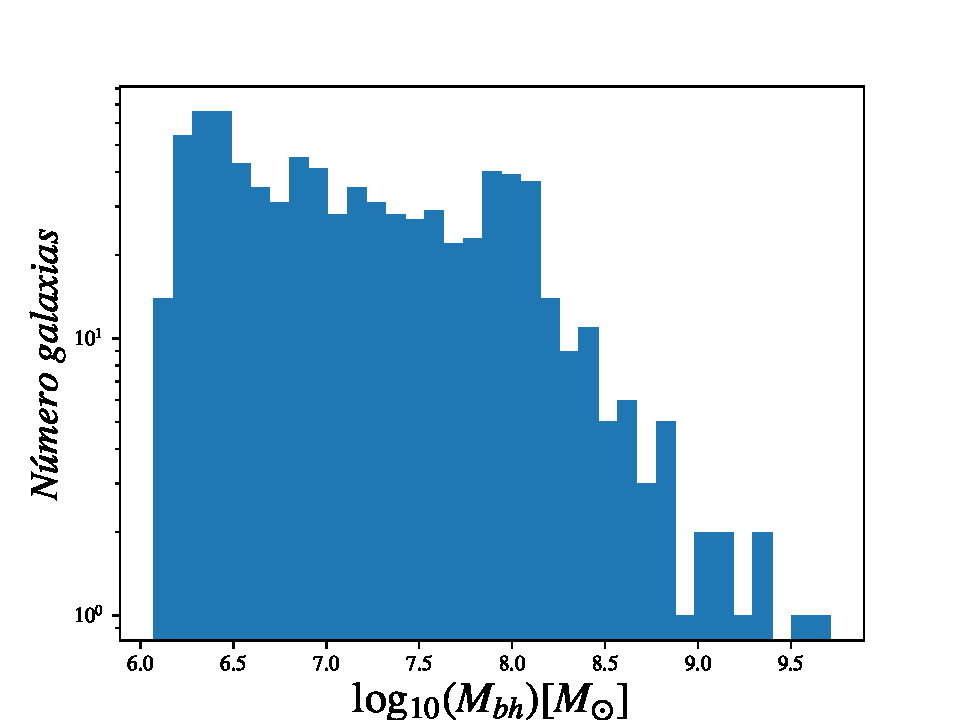
\includegraphics[width=0.32\textwidth]{./figures/6_Resultados/cosmo01/histo_Mass_bh.pdf}}
  \subfloat{
   %\label{fig: función de masa halos}
    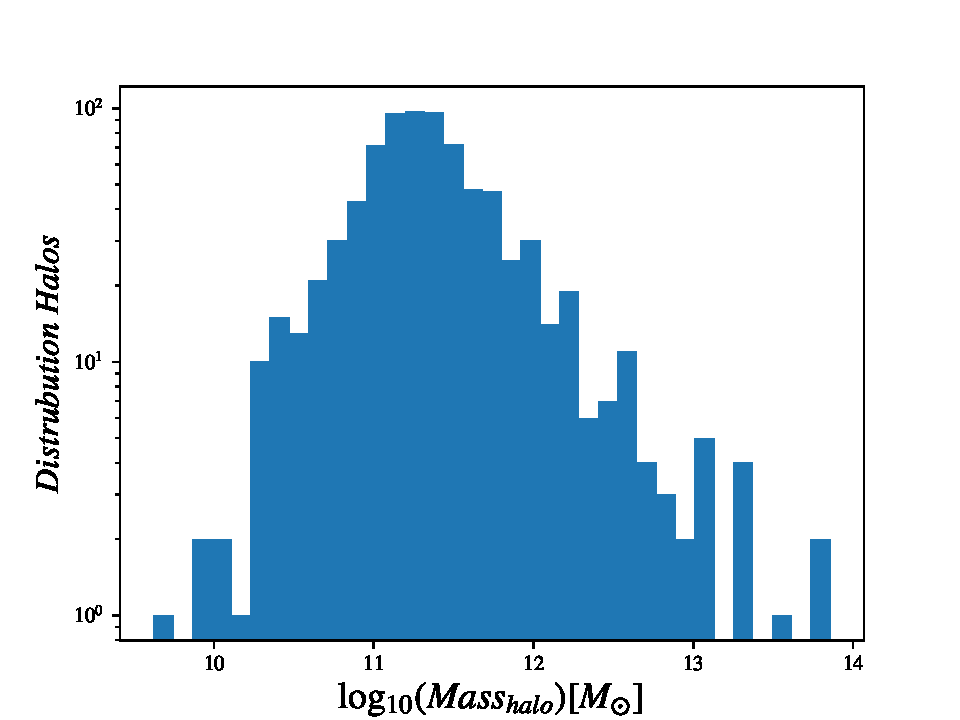
\includegraphics[width=0.32\textwidth]{./figures/6_Resultados/cosmo01/histo_Mass_halos.pdf}}
  \subfloat{
   %\label{fig: función de masa estelar}
    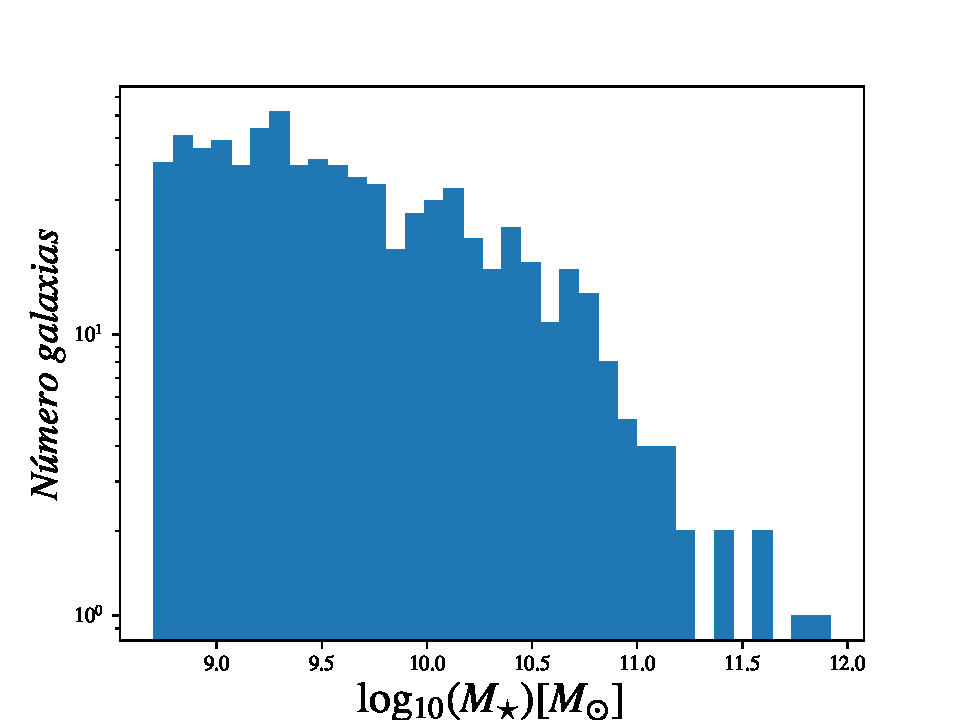
\includegraphics[width=0.32\textwidth]{./figures/6_Resultados/cosmo01/histo_Mass_stelar.pdf}}
 \caption{Funciones de masa para agujeros negros, halos y masa estelar, estas información da cuenta del número de objetos con una masa determinada, esto se realizo para {\it{Cosmo01}}. }
 \label{fig: Funciones de masa cosmo01}
\end{figure}
 %%%%%%%%%%%%%%%%%%%%%%%%%%%%%%%%%%%%%%%%%%%
 \begin{figure}
 \centering
  \subfloat{
   %\label{fig: función de masa BHs}
    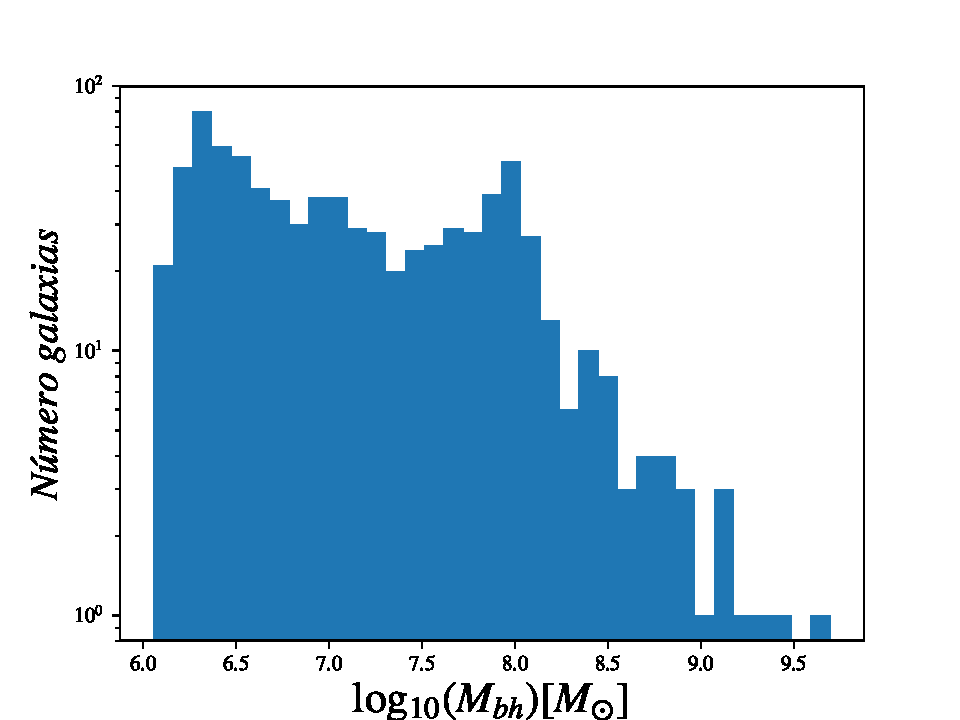
\includegraphics[width=0.32\textwidth]{./figures/6_Resultados/cosmo02/histo_Mass_bh.pdf}}
  \subfloat{
   %\label{fig: función de masa halos}
    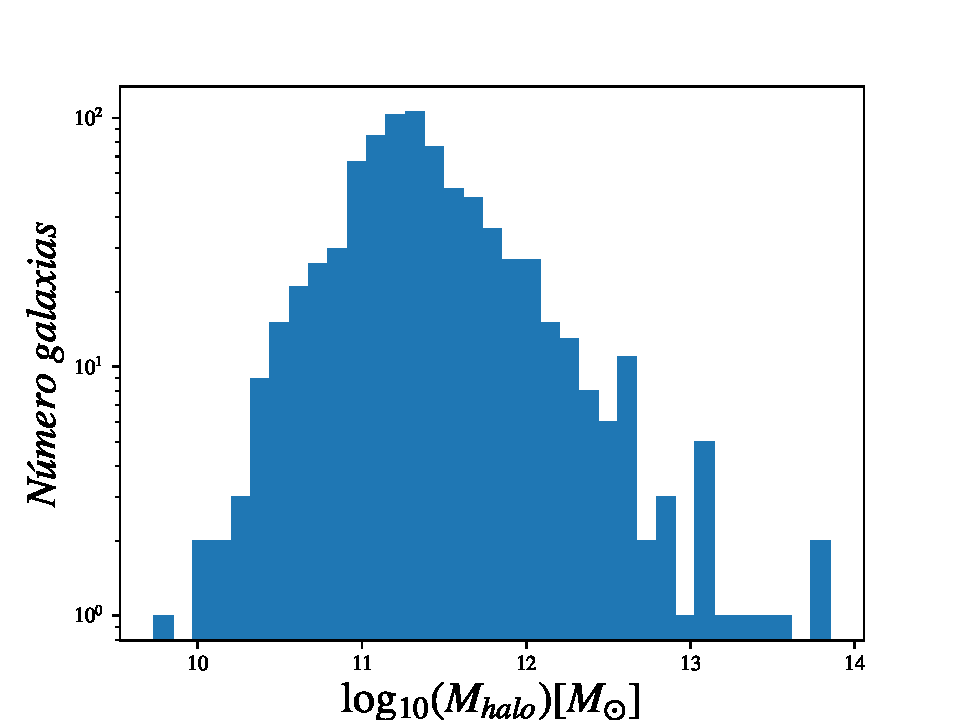
\includegraphics[width=0.32\textwidth]{./figures/6_Resultados/cosmo02/histo_Mass_halos.pdf}}
  \subfloat{
   %\label{fig: función de masa estelar}
    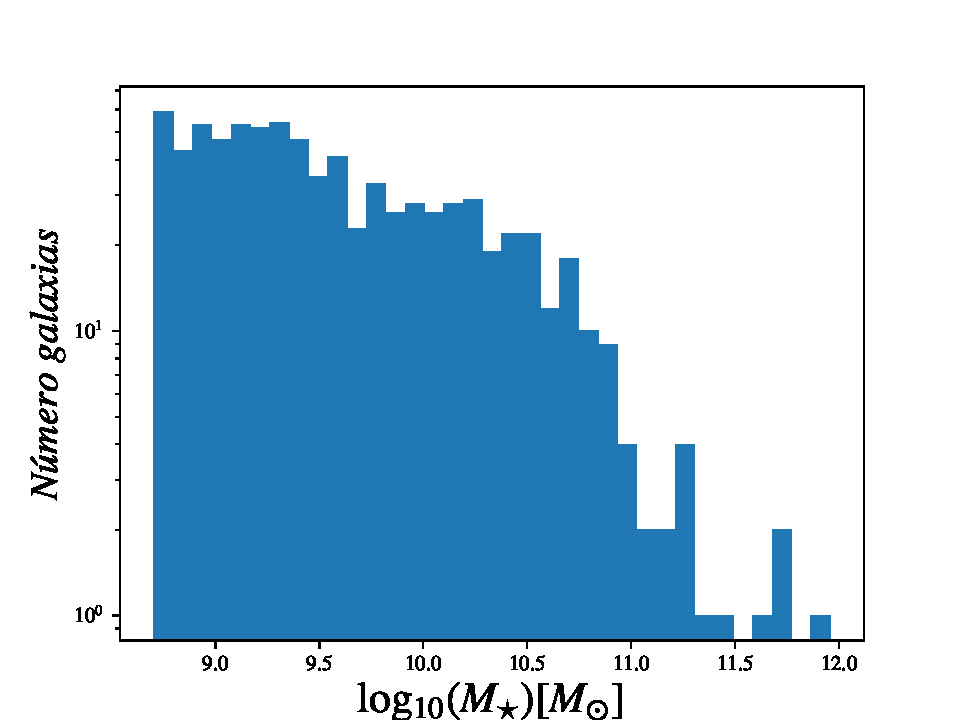
\includegraphics[width=0.32\textwidth]{./figures/6_Resultados/cosmo02/histo_Mass_stelar.pdf}}
 \caption{Funciones de masa para agujeros negros, halos y masa estelar, estas información da cuenta del número de objetos con una masa determinada, esto se realizo para {\it{Cosmo02}}.}
 \label{fig: Funciones de masa cosmo02}
\end{figure}
%
Al observar las figuras (\ref{fig: Funciones de masa cosmo01} y \ref{fig: Funciones de masa cosmo02}), es posible concluir que los resultados de la simulación son congruentes con la teoría y con las observaciones. Para despreciar los posibles errores producto de la baja resolución en galaxias de baja masa, se consideran sistemas en los cuales las masa estelar sea mayor a $5\times 10^{8}M_{\odot}$. Este criterio hace que la distribución de masa para los halos presente  esa extraña forma, con esta gráfica es posible argumentar que los halos de baja masa presentan una gran numero de masa estelar menor a $5\times 10^{8}M_{\odot}$, a medida que aumenta la masa del halo el numero de objetos con masa estelar menos al criterio disminuye. 

A parte de la función de distribución de masa es posible usar otros criterios que den información de la simulación y de su veracidad. 

La teoría sobre la formación de galaxias indica la existencia de una relación lineal entre la masa estelar de una galaxia y del BH anfitrión, por tanto las galaxias que poseen una masa estelar considerable poseen un BH con una masa considerable también. Por tanto las simulaciones debe reproducir este resultado teórico y observacional. Al observa las figuras (\ref{fig: Mass_bhVsMass_stelar}), es posible observar que las simulaciones bajo este criterio, también reproducen las observaciones. 
%
 \begin{figure}
 \centering
  \subfloat{
   %\label{fig: mass_bhVsmass_stelar}
    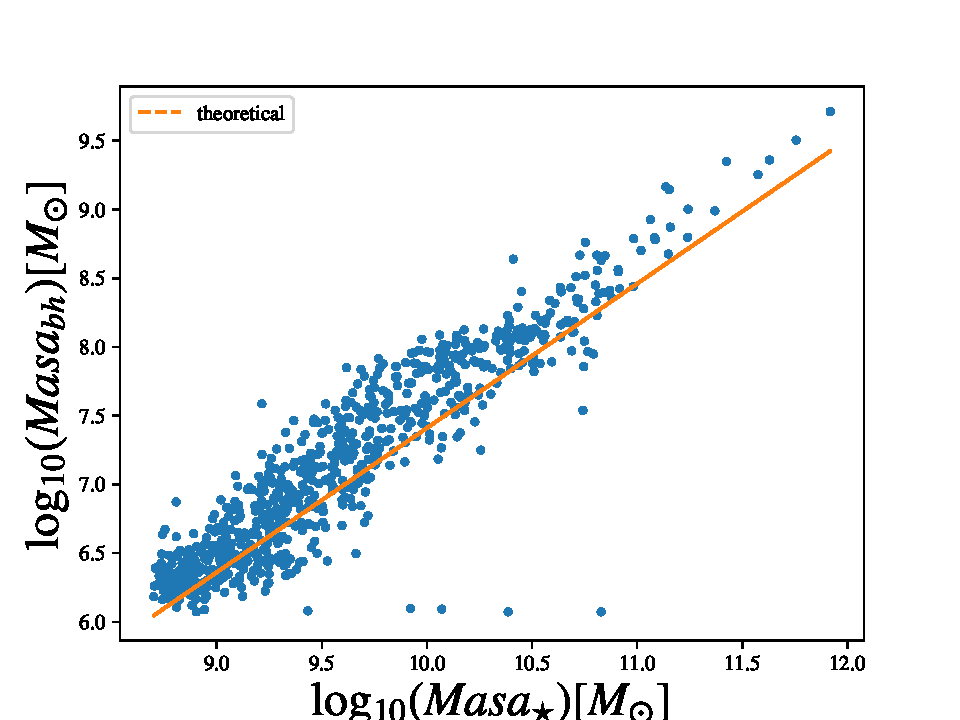
\includegraphics[width=0.49\textwidth]{./figures/6_Resultados/cosmo01/Mass_bhVsMass_stelar_halo.pdf}}
  \subfloat{
   %\label{fig: función de masa halos}
    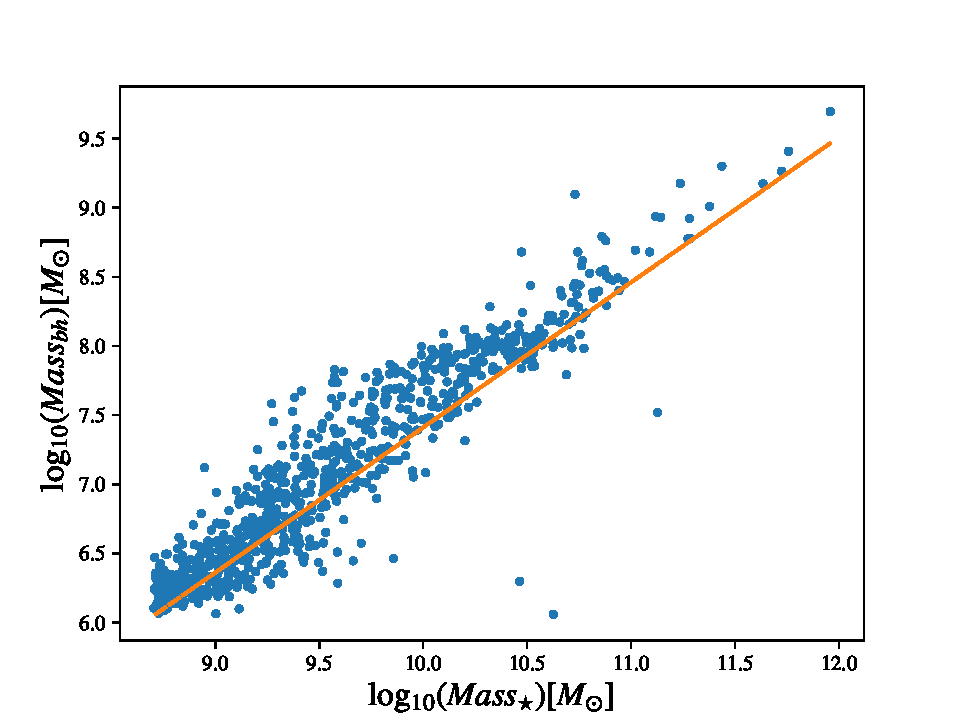
\includegraphics[width=0.49\textwidth]{./figures/6_Resultados/cosmo02/Mass_bhVsMass_stelar_halo.pdf}}
 \caption{Relación Masa BH y Masa estelar, según los resultados observacionales hay una dependencia lineal entre la masa del BH y la masa estelar para cada galaxia. La imágen de la derecha pertenece a {\it{cosmo01}} y el de la izquierda a {\it{cosmo02}}. La linea naranjada es la teórica\cite{McConnell2013}, con la cual se puede asegurar que la simulación es consistente con lo observacional.}
 \label{fig: Mass_bhVsMass_stelar}
\end{figure}
%
%------------------------------------------------
    \subsection{ Distribución de galaxias en el entorno cosmológico}
    \label{subsec: Distribucion de galaxias}
%------------------------------------------------

La distribución de las galaxias en el entorno cosmológico son determinantes en el resultado de final de este trabajo. Es necesario entonces poder concluir que los resultados obtenidos por las simulaciones reproduzcan las observaciones. Haciendo uso de método de T-Web, se extraen los autovalores $\lambda_{i}$, los autovectores $\vec{e}_{i}$ y la sobre densidad $\delta$. 

Como se explico en la sección (\ref{subsec: Metodo_T-web}),  los autovalores son los responsables de clasificar los entornos y con ello a las galaxias. Es necesario contrastar que la distribución de galaxias debe ser equivalente al mapa de sobre densidades. 

(ANALISIS Y GRAFICA DEL LA DENSIDAD CON )

Al observar las distribución de BHs en el espacio, se observa que gran parte de los BHs se ubica en los cluster o filamentos. Este resultado puede ser contrastado con el valores de los autovalores $\lambda_{i}$, al observar la figura (\ref{fig: Histograma Autovalores}) también se puede concluir lo siguiente:  $\lambda_{1}\geq 0$,  $\lambda_{2}\geq 0$ y $\lambda_{3}$ esta acotado entre $-10 \leq \lambda_{3}\leq 10$, mayormente con valores positivos, reproduciendo estructuras con características de filamentos o clusters. 
%
\begin{center}
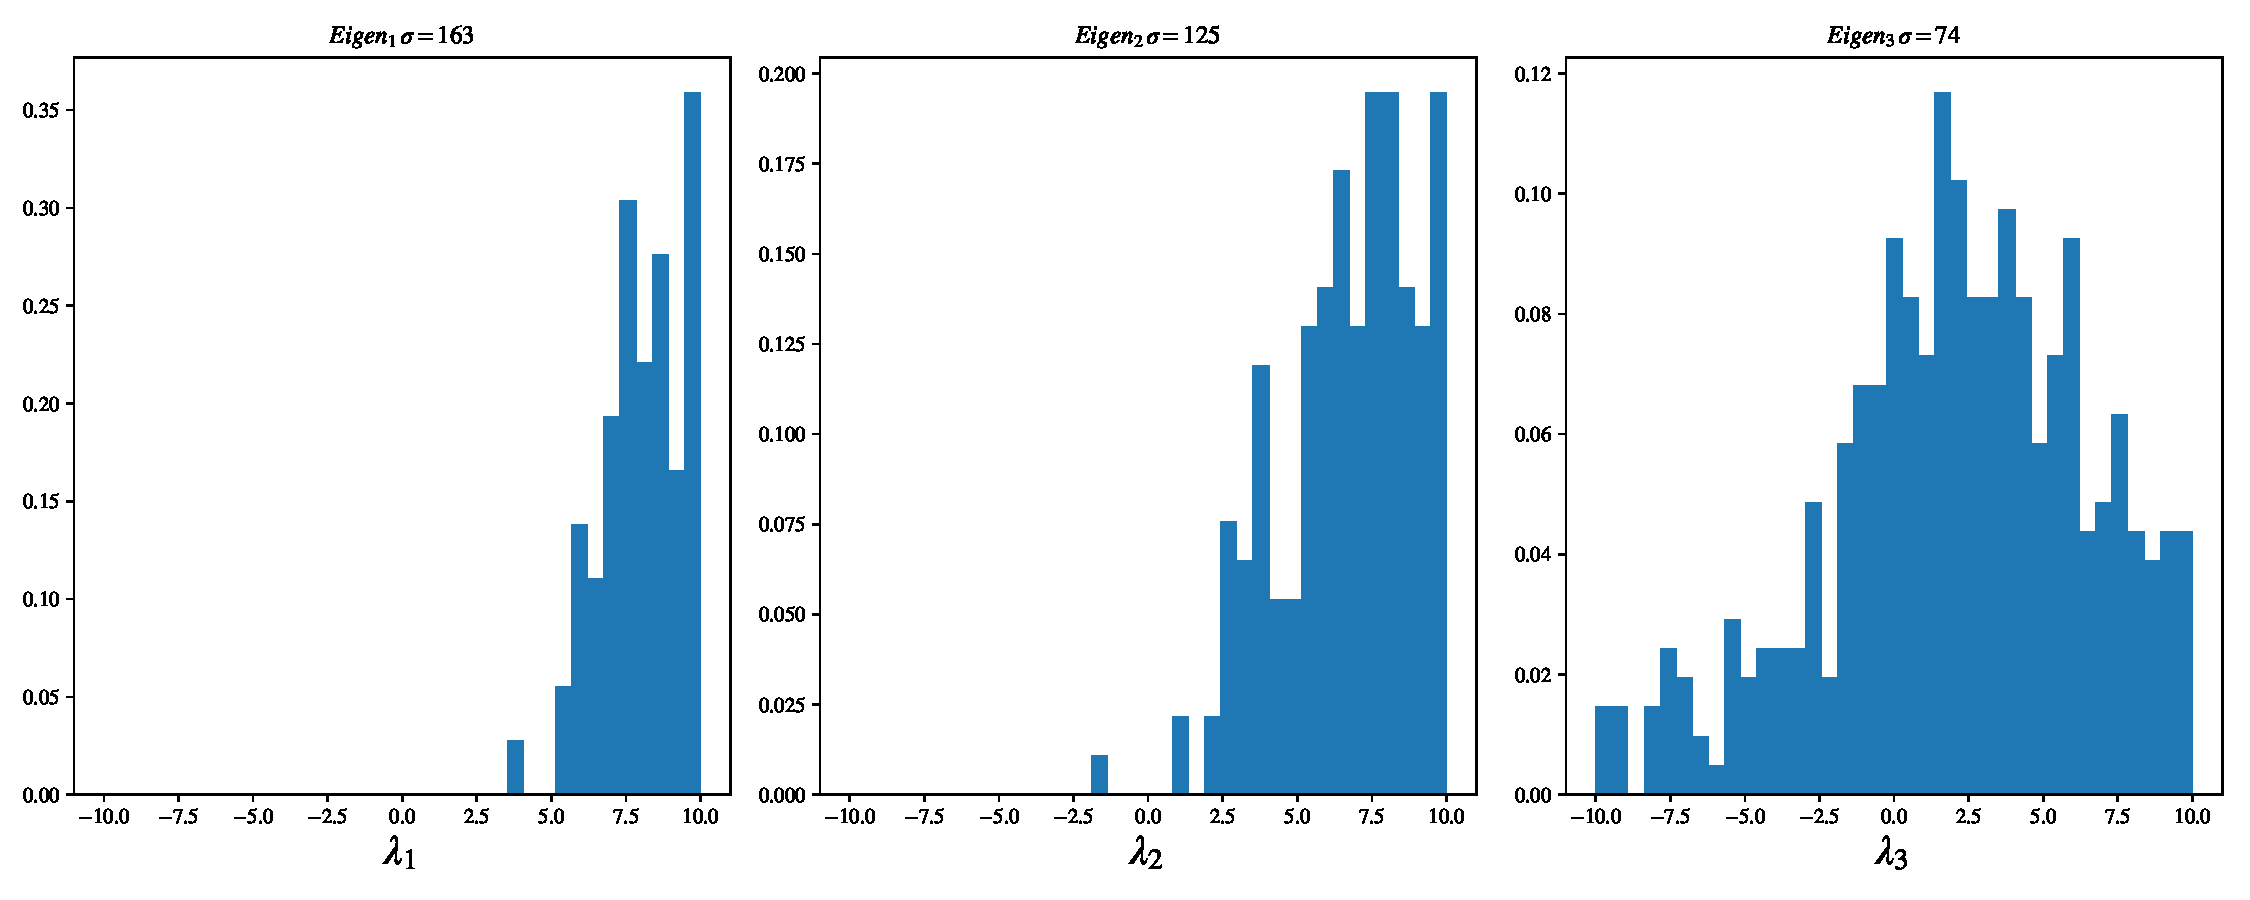
\includegraphics[scale=.38]{./figures/6_Resultados/cosmo01/histograma_autovalores2.pdf}
\figcaption{\emph{Histograma de los autovalores $\lambda_{i}$, que proporcionan información acerca de la clasificación y dinámica de la simulación a gran escala. Estos autovalores son obtenidos del método de  T-Web, calculando la diagonal de la matriz Hessiana.}}
\label{fig: Histograma Autovalores}
\end{center}
%




%------------------------------------------------
\section{ Alineamiento}
\label{sec: Alineamiento}
%------------------------------------------------

En esta sección se presentan los resultados que darán pie a argumentar si existe alguna relación entre el espín del BH y el entorno. Se mostraran los resultados logrados con varios sistemas (momentum angular de BHs, discos de acreción, halos y entorno), encaminados a comparar los resultados y poder dar respuesta a la pregunta planteada en este proyecto. 

Al recordando la estructuración de las galaxias, para la cual  se suponen galaxias con AGNs activos en su interior. Se consideran tres parámetros fundamentales para cada galaxia: en los halos se estudiará la masa estelar contenida en el halo, posición y momentum angular; para los AGN se estudiará el SMBH y el disco de acreción, del SMBH se extrae la masa, espín y posición y del disco de acreción el momentum angular. Estos parámetros fueron calculados usando la teoría de evolución de espín (ver capitulo \ref{cha:Modelo de Spin}) y usando el código {\it{Arepo}} (ver sección \ref{sec: codigo arepo} ) que reproduce la evolución y formación de galaxias. 

Para estudiar la alineación se utiliza como parámetro el $\cos (\theta)$, el cual está acotado entre -1 y 1 (ver sección \ref{subsubsec: Aling_Spin}). Partiendo de esto se argumenta que hay alineamiento sii  $\cos (\theta) \to 1$, anti-alineamiento si $\cos (\theta)\to -1$, ortogonalidad si $\cos (\theta)\to 0$ y si $\cos (\theta)\to \pm 0.5 $ no es posible concluir algo. Con base en esto se procede a calcular la relación entre los momentum angulares de cada sistema, a continuación se nombrar los ángulos con los cuales se busca encontrar alguna relación:

$\theta$ : ángulo entre el espín del BH ${\bf{J_{bh}}}$ y el autovector tres $\vec{\bf{e}}_{3}$.

$\alpha$ : ángulo entre el espín del BH ${\bf{J_{bh}}}$  y el disco de acreción ${\bf{J_{d}}}$ .

$\beta$ :  ángulo entre el espín del BH ${\bf{J_{bh}}}$ y el halos ${\bf{J_{halo}}}$

Una vez definidos los ángulos, procedamos a presentar una serie de resultados que contrastados con la teoría aportan a la solución de la respuesta central del texto. Como primera parte, identifiquemos cómo se comportan las alineaciones en la simulación, para esto se determinará la distribución de ángulos de alineamientos. 


(GRAFICAS HISTOGRAMAS DE ALPHA Y BETA)

En las gráficas () se puede concluir que gran parte de los espines de los BHs, discos de acreción y halos se terminan alineando. Esto puede inducir que los eventos de interacción son .....
%%%%*****************************************%%%%%%%%%%%%%%%
(HABLAR QUE DE AHORA EN ADELANTE SOLO SE VA HA CONSIDERAR COSMO01)
Valiéndonos de los resultados presentados en las simulaciones y de la teoría de alineamiento, se considera que la que mejor podría representar los sucesos "reales" o físicamnete más corectos es la simulación con acreción caótica. Por lo tanto a partir de acá los resultados reportados serán meramente resultados de {\it{cosmo01}}. 
%%%%%%%%%%%%%%%%%%%%%%%%%%%%%%%%%%%%%%%%%%%%%%%%%%%%%

Una vez visto estas relaciones, procedamos a estudiar como se comporta $\theta$. La relaciones que se obtengan de $\theta$ son de gran importancia, ya que está es la responsable de indicar si hay o no alineaminto con el entorno. Por tanto observemos que ocurre con la distribución de $\cos \theta$ para diferentes autovalores $\lambda_{i}$.
%
\begin{center}
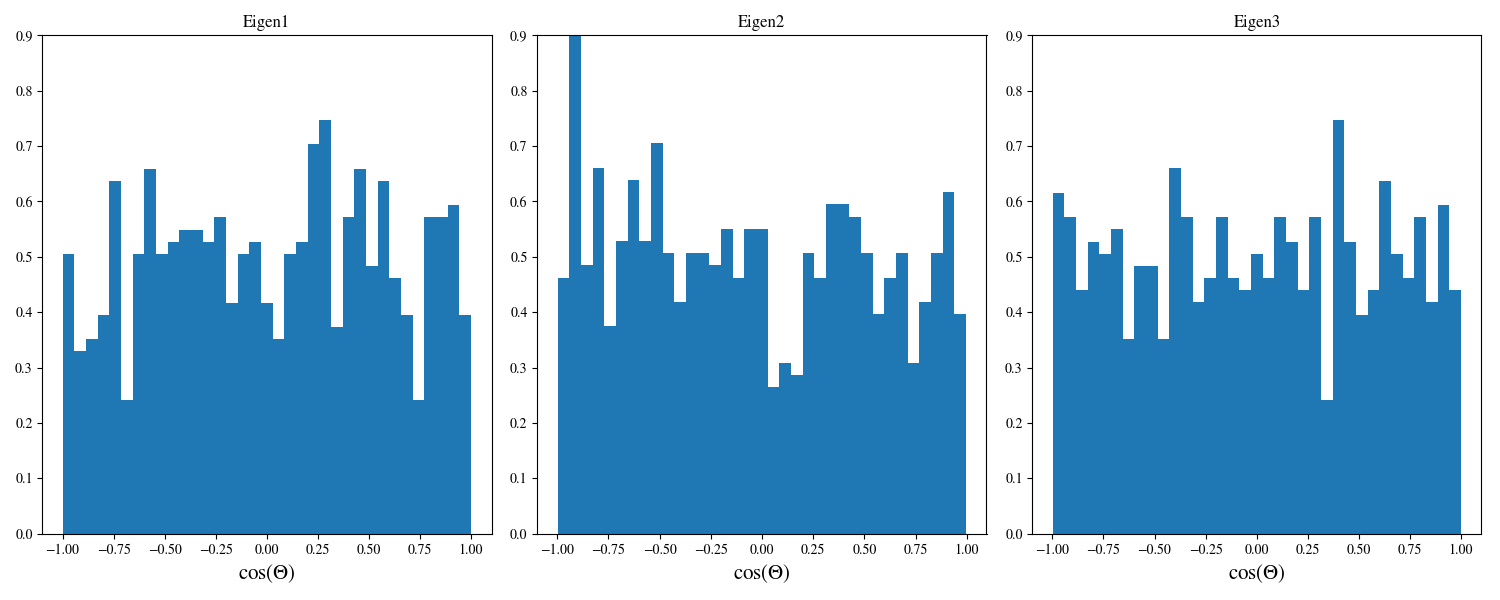
\includegraphics[scale=.35]{./figures/6_Resultados/cosmo01/histograma_cos_theta.png}
\figcaption{\emph{Distribución de $\cos \theta$ para cada BH en la simulación de cosmo01. Se observa una gran aleatoriedad debida que no se cuenta con un gran número de datos y porque se está considerando BHs alineados y no alineados.}}\label{fig: histograma costeta}
\end{center}
%
Al observar la figura (\ref{fig: histograma costeta}) se evidencia una gran aleatoriedad en la distribución de $\cos\theta$, la razón de ellos es que la distribución considera tanto BHs alineados como anti-alineados. Además se evidencia que para los tres autovalores ocurre lo mismo, una gran aleatoriedad. Para deshacernos de este problema se hace necesario estudiar el comportamiento de los BHs en regiones especificas de la simulación, donde se tenga alguna idea de un alineamiento.  

Ahora en búsqueda de no estimar objetos no alienados estudiemos entornos particulares, y ver si existe alguna relación entre el parámetro de alineamiento $\cos\theta$ y parámetros relacionados con el entorno, como lo son la masa del BH, la masa estelar del halo, masa del halo y autovectores, en especial $\lambda_{3}$. La teoría de formación de galaxias y estructuras muestra que en regiones de sobre densidad (clusters o filamentos) las galaxias presentan una mayor cantidad de masa  con respecto a las galaxias que se encuentran el regiones de baja densidad, lo cual se puede traducir en los BH de estas galaxias masivas también posee un gran cantidad de masa. Es entonces la masa el criterio usado para encontrar el posible alineamiento. 


\begin{figure} 
\centering \subfloat{ 
%\label{fig: función de masa BHs}
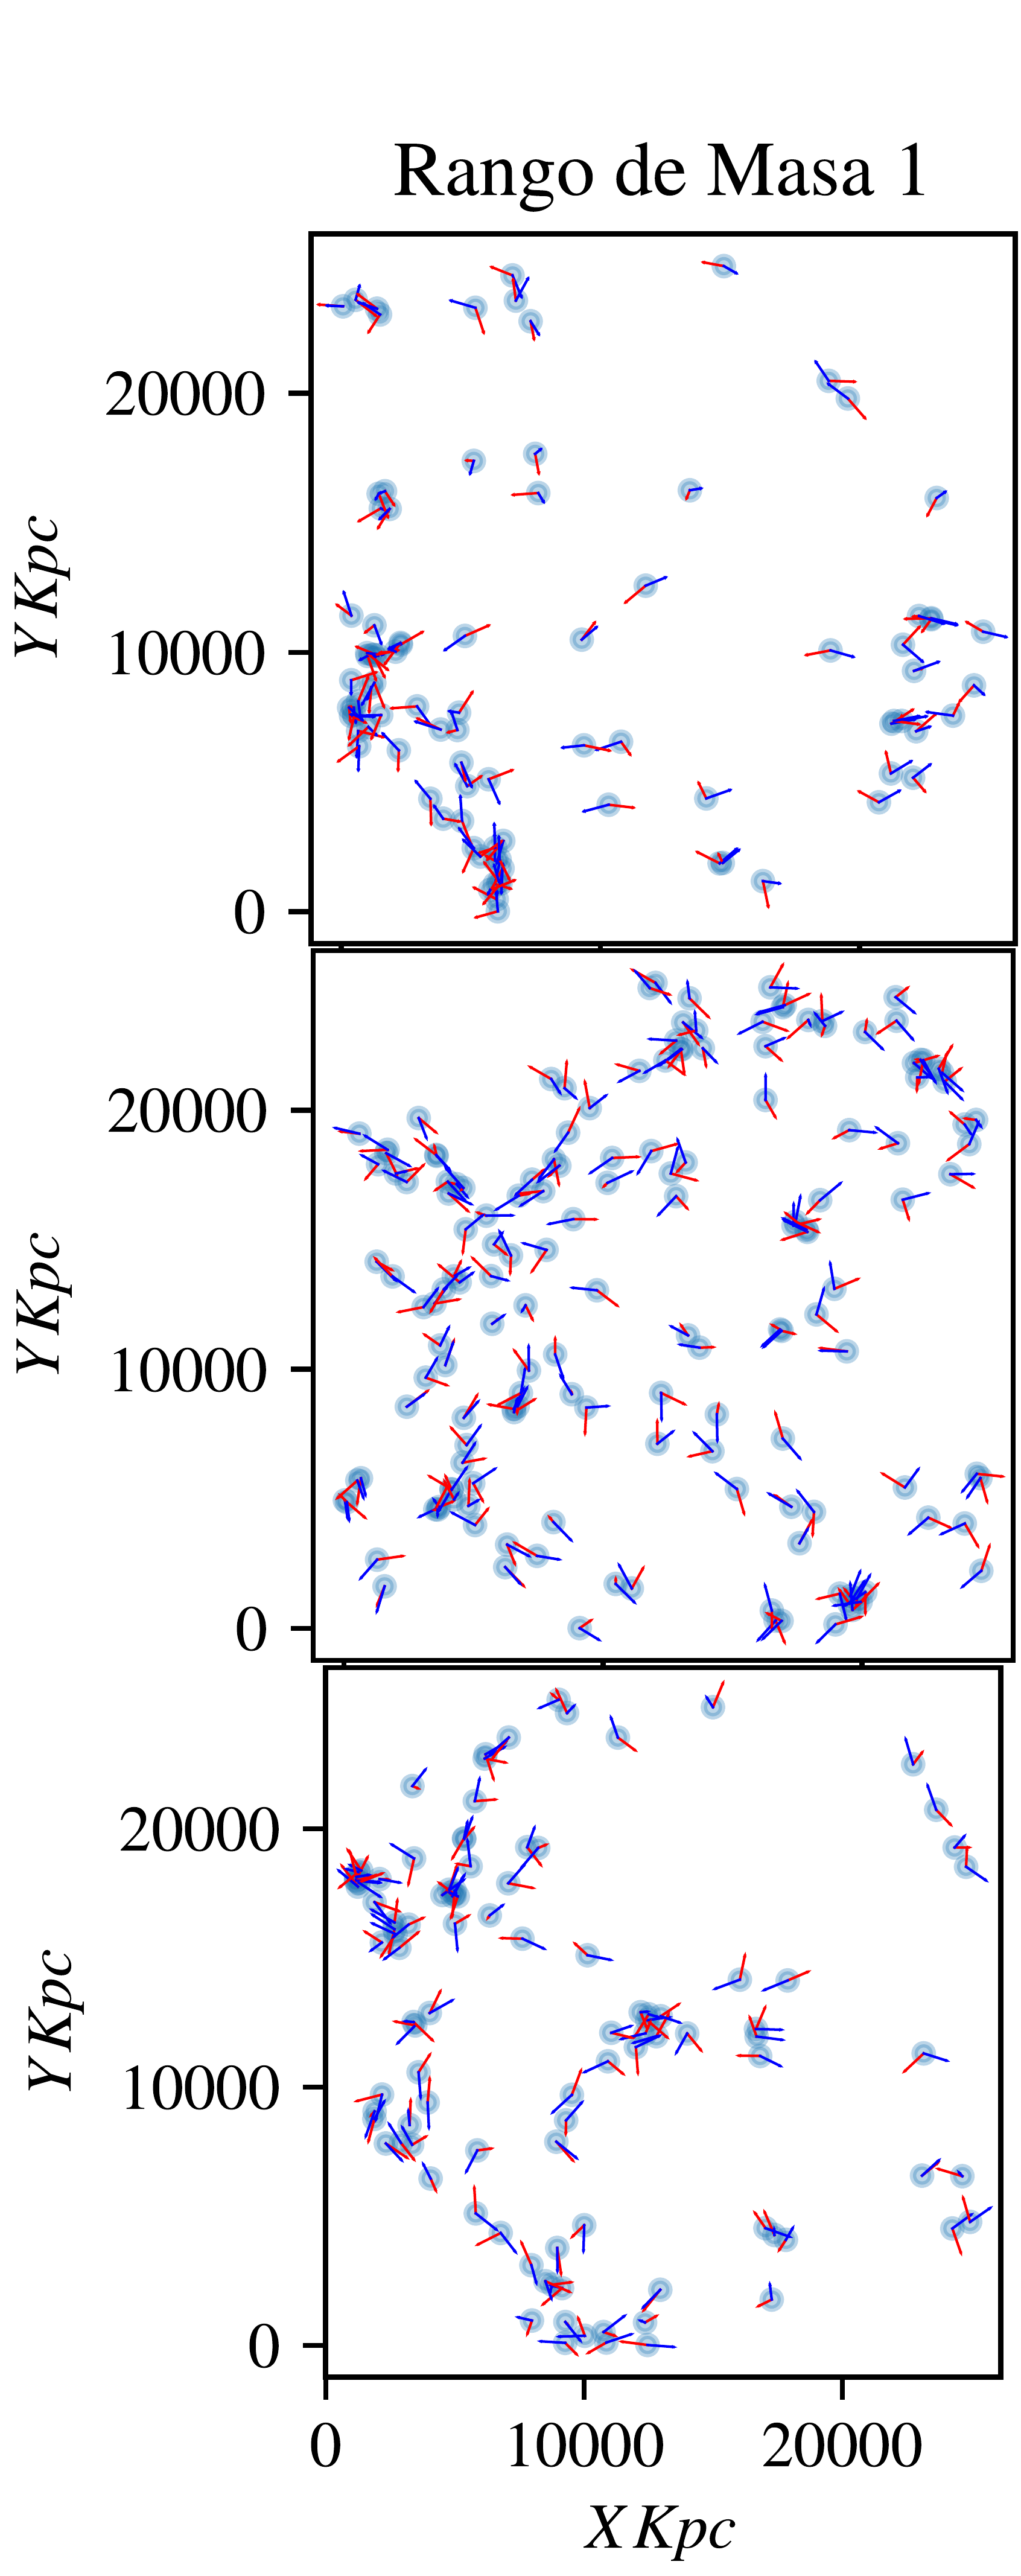
\includegraphics[width=0.38\textwidth]{./figures/6_Resultados/cosmo01/proyecion_rango_1_masas.png}} 
\subfloat{ 
%\label{fig: función de masa halos}
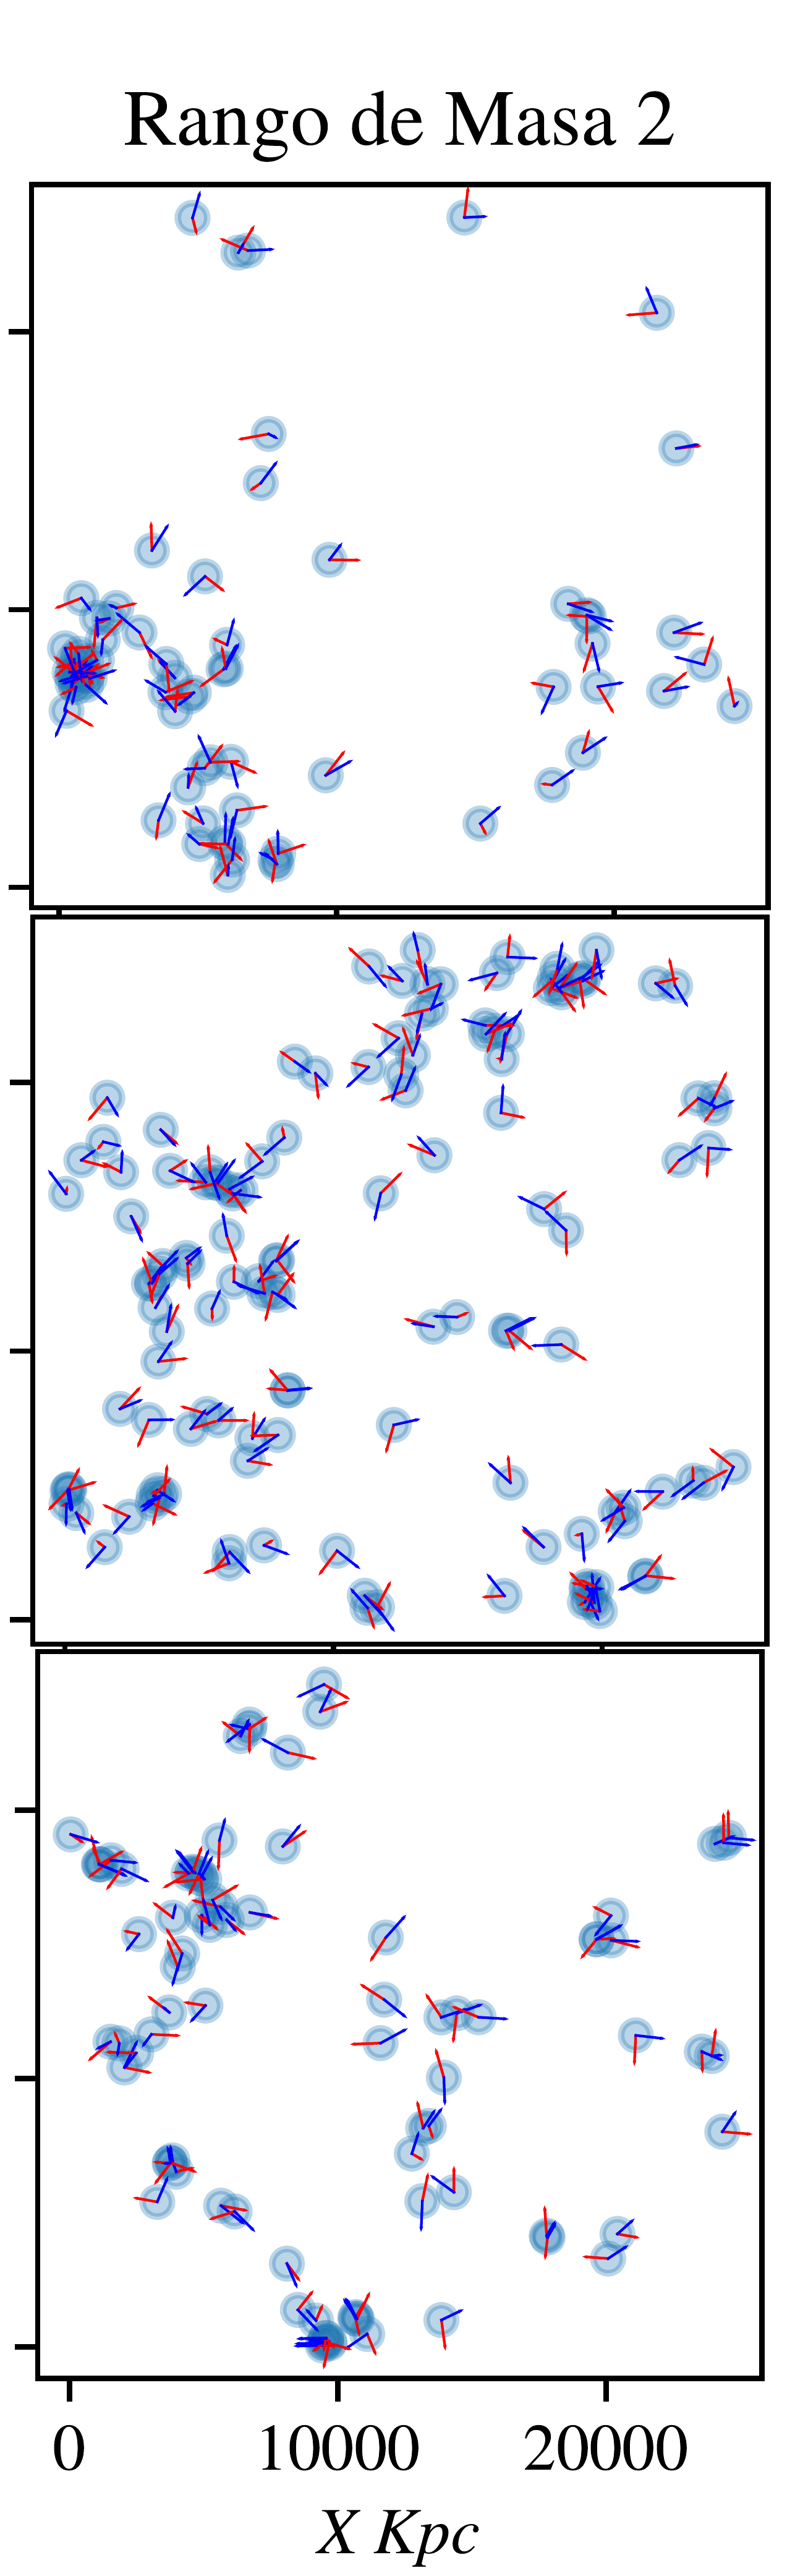
\includegraphics[width=0.29\textwidth]{./figures/6_Resultados/cosmo01/proyecion_rango_2_masas.png}}
\subfloat{
%\label{fig: función de masa estelar}
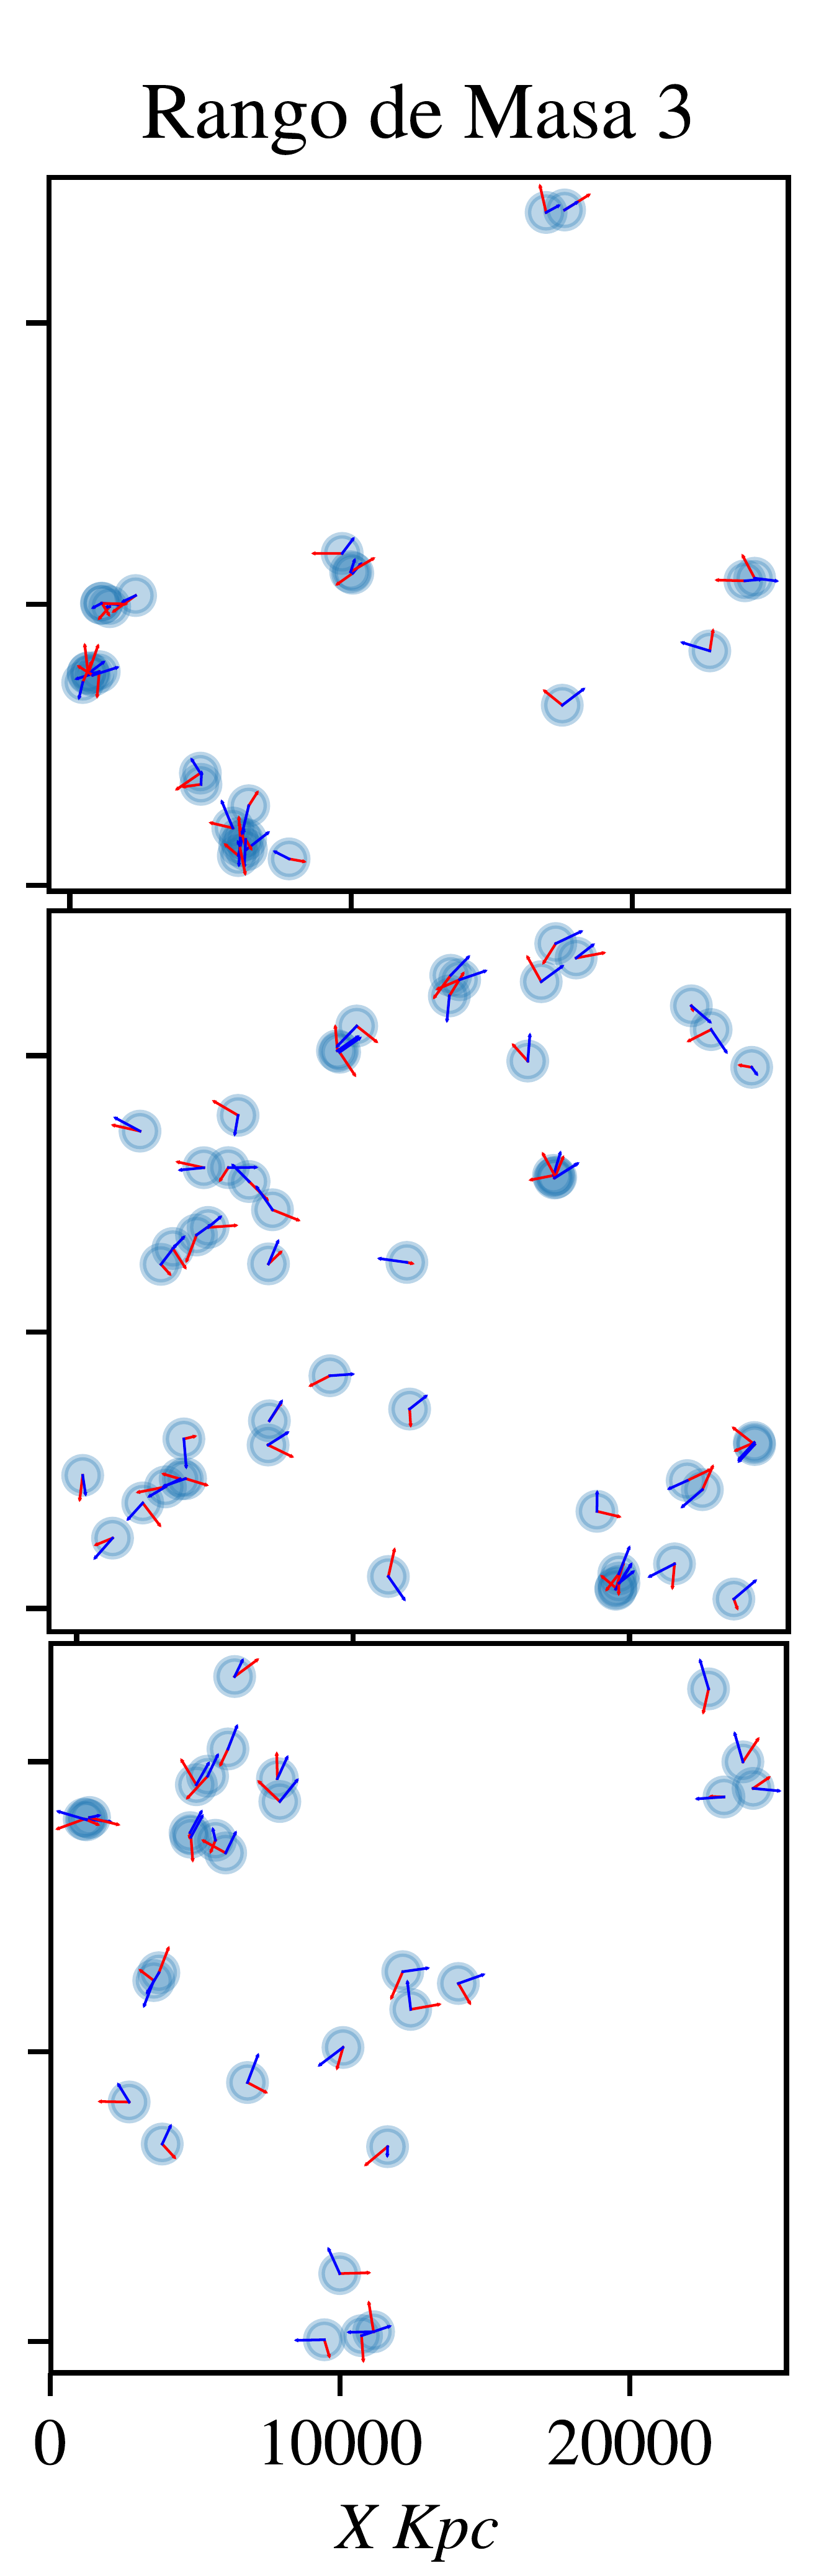
\includegraphics[width=0.302\textwidth]{./figures/6_Resultados/cosmo01/proyecion_rango_3_masas.png}} 
\caption{Representación de la correlación entre el autovector tres ${\bf{\vec{e}}_{3}}$ (Azul) y el espín del BH ${\bf{J_{bh}}}$ (Rojo). En esta figura se proyectan los vectores en el plano $x,y$. La figura presenta tres columnas, cada una de ellas relaciona un rango de masas, Rango 1 equivale a masas de BHs entre (6-7)/$M_{\odot}$, Rango 2 masas entre (7-8)/$M_{\odot}$ y Rango 2 masas entre (8-10)/$M_{\odot}$. Cada columna de rango consta de tres figuras, donde cada celda  representan tres cortes en la caja de la simulación, cortes hechos en el eje $z$, La primera fila indica un corte interior, BHs entre $(0, 8.3\times10^{3}) Kpc$,  la segunda fila un corte intermedio, entre $(8.3\times10^{3}, 16.6\times10^{3}) Kpc$, la ultima fila representa el corte superior, entre  $ (16.6\times10^{3}, 25\times10^{3}) Kpc$. } \label{} \end{figure}




%***********************************************************************



